\beginsong{Donna, donna}[wuw={Shalom Secunda, Aaron Zeitlin, 1940}, pfii={220}, pfiii={50}, gruen={271a}, index={On a wagon bound for market}]

\beginverse
\endverse
\centering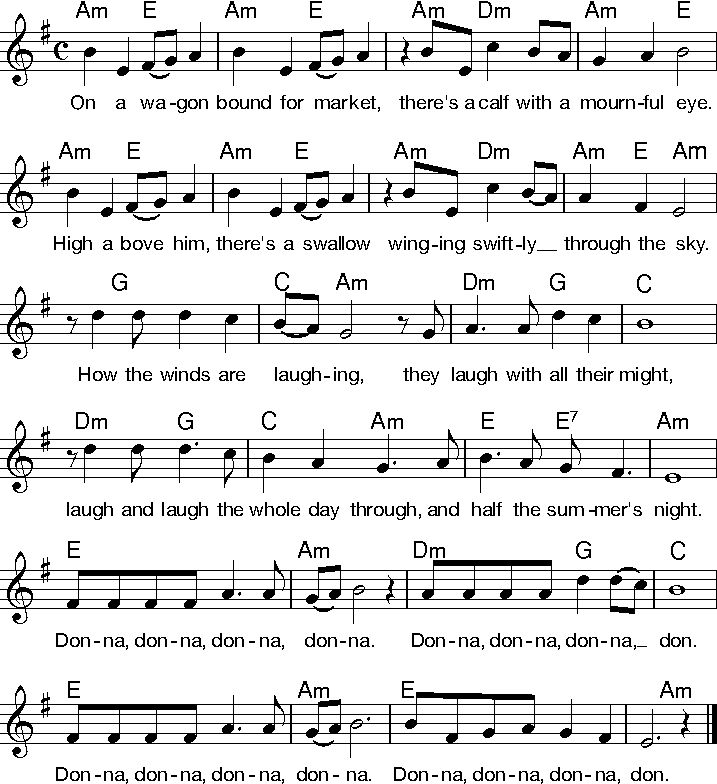
\includegraphics[width=1\textwidth]{Noten/Lied028.pdf}	

\beginverse
\[Am]''Stop com\[E]plaining'', \[Am]said the \[E]farmer. ''\[Am]Who told \[Dm]you a \[Am]calf to \[E]be? 
\[Am]Why can't \[E]you have \[Am]wings to \[E]fly with \[Am]like the \[Dm]swallows so \[Am]proud \[E]and \[Am]free?''
\endverse

\beginchorus
\[G]How the winds are \[C]laugh\[Am]ing, they \[Dm]laugh with \[G]all their \[C]might,
\[Dm]laugh and \[G]laugh the \[C]whole day \[Am]through and \[E]half the \[E7]summer's \[Am]night.
\[E]Donna, donna, donna, \[Am]donna. \[Dm]Donna, donna, \[G]donna, \[C]don.
\[E]Donna, donna, donna, \[Am]donna. \[E7]Donna, donna, donna, \[Am]don.
\endchorus

\beginverse
^Calves are ^easily ^bound and ^slaughtered, ^never ^knowing ^the reason ^why. 
^Whoever ^treasures ^freedom ^like the ^swallow ^has ^learned ^to ^fly.
\endverse

%\renewcommand{\everychorus}{\textnote{\bf Refrain (wdh.)}}
\beginchorus
\[G]How the winds are \[C]laugh\[Am]ing, they \[Dm]laugh with \[G]all their \[C]might,
\[Dm]laugh and \[G]laugh the \[C]whole day \[Am]through and \[E]half the \[E7]summer's \[Am]night.
\[E]Donna, donna, donna, \[Am]donna. \[Dm]Donna, donna, \[G]donna, \[C]don.
\[E]Donna, donna, donna, \[Am]donna. \[E7]Donna, donna, donna, \[Am]don.
\endchorus

\endsong

\beginscripture{}
Das Lied berichtet von der Behandlung der Juden zur Zeit des NS-Regimes. Es handelt von einem Kälbchen, das sich dagegen wehrt, zur Schlachtbank geführt zu werden. „Donna“ kommt vom hebräischen Wort „Adonai“, einer üblichen Anrede Gottes. Das Lied wurde ursprünglich in der jüdischen Sprache für das Musical ''Esterke'' (1941-1942) verfasst.
\endscripture
